\documentclass[ThesisDJ.tex]{subfiles}

\begin{document}

In diesem Kapitel geht es um die Plannung des Projekts. Die Planungsphase gehört zu den wichtigsten Phasen des Projektmanagements. Hier werden finanzielle Mittel, Zeitplan und das vorhandene Personal zusammengefasst und der Projektplan erstellt. An diesem orientieren sich die Beteiligten während des gesamten Projekts, was die Relevanz dieser Phase unterstreicht. Die Planungsphase wird dazu genutzt, um die Strukturen im Projekt aufzubauen. Dazu zählt das Verteilen von Rollen und Verantwortungen im Projekt. Weiterhin müssen Kommunikationswege implementiert und Eskalationswege definiert werden. 
Zudem werden Meilensteine benannt und festgelegt, sowie die Arbeitspakete erstellt, um die Meilensteine zu erreichen. Eine ausführliche Risiko-Analyse ist auch Teil dieser Phase. 

\subsection{Arbeitspakete und Meilensteine (NW)}
In einem Projekt werden die Aufgaben in verschiedene Einheiten unterteilt. Diese sind Hierarisch angeordnet. Typischerweise wird zwischen Meilensteinen und Arbeitspaketen unterschieden.
Ein Meilenstein besteht hierbei aus mehreren Arbeitspaketen.

\subsubsection{Arbeitspakete (NW)}
Arbeitspakete teilen die Arbeit im Projekt in kleinere, überschaubare Aufgaben ein. Sie stellen die kleinste Einheit im
Projektstrukturplan dar und helfen dabei den Zustand des Projekts zu bewerten.
Ein Arbeitspaket hat ein klares Ziel, sowie definierte Start- und Endtermine, sowie einen defnierten Arbeitsumfang. 
Zusätzlich können Arbeitspakete in Abhängigkeit von anderen Paketen definiert werden und benötigte Ressourcen sowie 
eine Definition enthalten ab wann ein Paket als abgeschlossen gilt. Auch Verantwortlichkeiten können zugeordnet werden. 
Arbeitspakete können dabei verschiedene Zustände haben. Eine Möglichkeit ist es den Paketen einen Diskreten Zustand 
zuzuordnen. Typischerweise wird unterschieden zwischen nicht bearbeitet, in Bearbeitung und abgeschlossen. Es kann jedoch auch 
Sinnvoll sein den Bearbeitungszustand in Prozent anzugeben. Dies setzt allerdings eine sinnvolle Metrik voraus. 

\paragraph{Arbeitspaketbestimmung (NW)}
Bestimmt wurden die Arbeitspakete von den Projektmitarbeitern. Dabei haben alle Projektmitarbeiter unabhängig Arbeitspakete 
formuliert. Diese wurden dann zusammengetragen und ergänzt oder zusammengefasst.
Die Arbeitsaufwandschätzung wurde mit der Mittelwertmethode ermittelt. Dabei schätzen die Projektmitarbeiter den Aufwand für ein 
Arbeitspaket. Aus diesen Werten wird dann der Mittelwert bestimmt. Dieser wird dann als Aufwand für das Arbeitspaket angenommen. 
Da das Team sehr unerfahren mit dem Planen von Projekten ist, eignet sich diese Methode besonders gut, wenn man davon ausgeht 
dass die Schätzungen um den reellen Aufwand herum liegen. Durch den Mittelwert lassen sich nun abweichungen schmälern. Dabei 
werden natürlich bessere Ergebnisse erziehlt, je mehr Personen mitschätzen. 

\subsubsection{Meilensteine (NW)}
Meilensteine in einem Projekt markieren den Abschluss eines bestimmten Ziels. Meistens werden diese auf ein bestimmtes Datum festgelegt.
Sie dienen Dazu den Überblick in einem Projekt zu beahlten und den Verlauf des Projekts besser einschätzen zu können. 
Außerdem können diese als Motivator dienen, wenn ein gesetztes Ziel eingehalten werden kann. 
Auch die Meilensteine wurden zusammen festgelegt.


\subsection{Organisation und Kommunikation (NW)}
Das Projekt wird von 3 Projektmitarbeitern bearbeitet. Als Ansprechpartner dient ein Mitarbeiter des gleichen Unternehmens. Die Projektmitarbeiter bearbeiten das Projekt wöchentlich an ihrem Praxistag. Zudem wird wöchentlich ein Meeting abgehalten, welches dazu dient, sich gegenseitig auf den aktuellen Stand zu bringen und eventuelle Anpassungen an der Planung vorzunehmen. Weitere Absprachen mit Abteilungs- und Bereichsleitern werden nach Bedarf organisiert. In der Regel richten sich diese nach den Meilensteinen des Projekts.  

\subsection{Ressourcen (NW)}

Die Ressourcen umfassen die Arbeitskraft, die diesem Projekt zur Verfügung steht, sowie Räumlichkeiten. 
Die verfügbare Arbeitskraft berechnet sich aus der Anzahl der Mitarbeiter mulitipliziert mit den jeweiligen Personenstunden.
In diesem Projekt sind drei Projektmitarbeiter welche jeweils eine Arbeitskraft von 8 Personenstunden pro Woche in das Projekt einbringen. 
Die Resultiernede Arbeitskraft entspricht damit:

		\emph{8 Personenstunden x 15 Tage x 3 = 360 Personenstunden}\\
Weiterhin wurde den Studierenden ein Raum vor Ort zur Verfügung gestellt. Diese Räume beinhalten benötigte Medien, um ein gemeinsames arbeiten zu ermöglichen.

\subsection{Kommunikationsmanagement (JD)}
Ein effektives Kommunikationsmanagement stellt einen wesentlichen Erfolgsfaktor im Projektmanagement dar, da es sicherstellt, dass alle relevanten Informationen zielgerichtet und zeitnah an die richtigen Stakeholder übermittelt werden.

\subsubsection{Theoretische Grundlagen Kommunikationsmanagement (JD)}}
 Gemäß dem PMBOK Guide umfasst das Kommunikationsmanagement die Planung, Verteilung, Erfassung und Speicherung von Informationen sowie das abschließende Reporting \cite{PMI2017PMBOK}. Hierbei gilt es, die Bedürfnisse der verschiedenen Gruppen – vom internen Projektteam bis hin zu externen Auftraggebern – zu identifizieren und entsprechende Kommunikationskanäle sowie -formate festzulegen.

Schwalbe hebt in ihrem Werk \emph{Information Technology Project Management} hervor, dass ein wirksamer Kommunikationsplan nicht nur die Auswahl der geeigneten Kommunikationswege, sondern auch die Festlegung von Meetingstrukturen, Berichtszyklen und Eskalationspfaden beinhalten muss \cite{Schwalbe}. Durch diese systematische Herangehensweise wird gewährleistet, dass Unklarheiten vermieden und Entscheidungen auf einer fundierten Informationsbasis getroffen werden können.

Ergänzend betont Kerzner in \emph{Project Management: A Systems Approach to Planning, Scheduling, and Controlling} die Notwendigkeit standardisierter Kommunikationsprozesse. Eine klare Struktur mit einheitlichen Berichtsformaten und definierten Verantwortlichkeiten erleichtert die kontinuierliche Überwachung des Projektfortschritts und erlaubt es, frühzeitig auf Abweichungen zu reagieren \cite{Kerzner}. Gerade in der Planungsphase trägt die präzise Dokumentation aller Kommunikationsaktivitäten maßgeblich zur Reduktion von Unsicherheiten bei.

Moderne IT-Tools wie cloudbasierte Kollaborationsplattformen, Instant-Messaging-Dienste und virtuelle Meeting-Tools erweitern diese klassischen Ansätze um eine hohe Flexibilität und ermöglichen den Echtzeit-Austausch von Informationen – ein besonders wichtiger Aspekt in dynamischen und verteilten Projektumgebungen \cite{GPM}.

Zusammenfassend lässt sich festhalten, dass ein gut strukturierter Kommunikationsplan durch die Integration bewährter Konzepte und moderner Technologien wesentlich zur Planungssicherheit und zum Projekterfolg beiträgt.

\subsubsection{Arten und Methoden der Kommunikation (JD)}

 \begin{table}
	\begin{tabular}{|p{3cm}|p{6.5cm}|p{6.5cm}|}
		\hline 
		Typ & Formell & Informell\\
		\hline
		Verbal & 
		\begin{tabular}{l}
			Präsentationen\\
			Projekt-Reviews\\
			Briefings\\
			Produktdemonstrationen\\
			Brainstormings
		\end{tabular} & 
		\begin{tabular}{l}
			Konversationen\\
			Ad-hoc Diskussionen
		\end{tabular}\\
		\hline
		Schriftlich &
		\begin{tabular}{l}
			Fortschrittsberichte\\
			Projektdokumentationen\\
			Geschäftsideen
		\end{tabular} & 
		\begin{tabular}{l}
			Kurze Notizen\\
			E-Mails\\
			Messenger (WhatsApp,\\ Telegram, Signal usw.)\\
			Soziale Medien
		\end{tabular}\\
		\hline
	\end{tabular}
	\caption{Kommunikationstypen. Entnommen aus \cite[S.~108]{PMI2017PMBOK} Abb. 2.1 (JD)}
	\label{tab:comm_methods}
\end{table}

Der PMBOK Guide \cite[S.~108]{PMI2017PMBOK} beschreibt verschiedene Arten der Kommunikation mit Stakeholdern. Wie in Tabelle \ref{tab:comm_methods} dargestellt, lässt sich Kommunikation nach zwei Kriterien kategorisieren: dem Medium der Kommuniktion und dem Level an Förmlichkeit, also der Unterscheidung zwischen formeller und informeller Kommunikation.\\
Kombiniert man beide Kriterien zu einer Matrix, wie in der Tabelle dargestellt, ergeben sich daraus die folgenden Kommunikationswege:
\begin{itemize}
	\item \emph{Verbal und Formell:}\\
	Präsentationen, Projekt-Reviews, Briefings, Produktdemonstrationen, aber auch Brainstormings sind Kommunikation, die primär verbal stattfindet und dabei förmlich strukturiert ist. Das involviert auch eine Vorherige Planung eines Termins zur Durchführung und eine Vorbereitung der Teilnehmer auf den Termin.
	\item \emph{Verbal und Informell:}\\
	Einfache Konversationen und spontane Ad-hoc Diskussionen sind ebenfall primär verbale Wege der Kommunikation, allerdings in einem informellen Rahmen. Hier findet keine Planung oder Terminfindung statt, ebenso sind die Teilnehmer in der Regel nicht für diesen konkreten Termin vorbereitet, sondern es findet ein offener Austausch an Informationen statt.
	\item \emph{Schriftlich und Formell:}\\
	Fortschrittsberichte, Projektdokumentationen und Geschäftsideen sind Arten der förmlichen Kommunikation, die in schriftlicher Form ausgeführt wird. Diese Dokumente sind oft formalisiert und folgen vereinbarten Regeln, müssen in bestimmten Abständen erneut vorgelegt werden, oder haben einen vorher fest vereinbarten Rahmen und Inhalt.
	\item \emph{Schriftlich und Informell:}\\
	Einfache Notizen, E-Mails, Nachrichten über Messenger wie WhatsApp, Telegram oder Signal sowie Nachrichten über Soziale Medien sind ebenfalls in Schriftform, allerdings in der Regel nicht besonders reglementiert und eine Kommunikation findet eher spontan statt. 
\end{itemize}
Neben den Medien, die zur Kommunikation eingesetzt werden, lässt sich Kommunikation auch danach klassifizieren, von welcher Seite sie ausgeht. Dabei werden folgende Begriffe eingesetzt:
\begin{itemize}
	\item \emph{Push-Kommunikation:}\\
	Bei der Push-Kommunikation werden Informationen vom Projekt-Team an die Stakeholder auf in der Regel vorher definierten Wegen direkt übermittelt. Es kann sich dabei um verbale oder schriftliche und formelle oder informelle Arten der Kommuniktion handeln, wichtig ist, dass die Informationen in der Regel nur in eine Richtung (zu den Stakeholdern) fließen und nur beschränkt Rücksicht darauf genommen wird, ob die Stakeholder in diesem Moment eigentlich in der Lage sind, diese Informationen auch zu verarbeiten. Diese Methode ermöglicht eine schnelle und direkte Information von vielen Stakeholdern, sollte aber aufgrund der Nachteile mit Bedacht eingesetzt werden.
	\item \emph{Pull-Kommunikation:}\\
	Bei der Pull-Kommunikation werden Informationen vom Projekt-Team an für die Stakeholder erreichbaren Orten bereitgestellt. Die Stakeholder können dann, wenn sie die Kapazitäten dazu haben, diese Informationen einsehen und damit zu arbeiten. Dieser Ansatz ist flexibler als die Push-Kommunikation, da Stakeholder nur dann Nachrichten abrufen, wenn sie sie gerade benötigen. Außerdem ermöglicht ein zentraler Ablageplatz der Informationen auch ein langfristiges Management der abgelegten Informationen inklusive der Möglichkeit, bei Änderungen am Projekt entsprechende Informationen in der Ablage zu verändern, ohne alle Stakeholder unmittelbar darüber informieren zu müssen.
\end{itemize}

\subsubsection{Kommunikation im realen Projekt (JD)}
Die Kommunikation mit den Stakeholdern im untersuchten Projekt gestaltet sich entsprechend der Projektgröße und der Bedeutung für den Bereich J3 bzw. die HZD verhältnismäßig simpel.\\
Die allgemeine Kommunikation im Bereich J3 ist, sowohl innerhalb der einzelnen Verfahrens- bzw. Projekt-Teams als auch zwischen den Teams und mit der Bereichsleitung nach Möglichkeit informell gestaltet. Bei entsprechenden Vorgaben, der Kommunikation mit anderen Bereichen oder der Notwendigkeit einer formell sauberen Nachverfolgbarkeit von Entscheidungen und Aktivitäten, werden formelle Wege der Kommunikation (und Dokumentation) genutzt, darüber hinaus werden viele Informationen über spontane Unterhaltungen und Diskussionen vermittelt.\\
Um dieser Praxis zu folgen werden auch im betrachteten Projekt nur notwendige Schritte formell durchgeführt. Dies beinhaltet neben dem Projekt-Kickoff und dem Projekt-Abschluss vor allem die festgelegten Ergebnisse des Projekts, also die Software-Evaluation und (ursprünglich) der Proof-of-Concept inklusive Dokumentation.\\
Weitere Kommunikation inklusive der Information der Stakeholder bei Fortschritten oder Veränderungen im Projekt erfolgt in der Regel informell bei spontanen Gesprächen.\\
Die Stakeholder, die ein Interesse an den konkreten Ergebnissen und ermittelten Informationen des Projekts haben, haben zudem einen Zugang auf verschiedene Informationsablagen des Projektteams, womit in diesen Bereichen eine Pull-Kommunikation umgesetzt wird.

\section{Risikomanagement (LL)}
Ein essenzieller Bestandteil der Projektplanung ist die Risikoanalyse, da eine Projektplanung zwar sehr akkurat und organisiert sein kann, jedoch unter Umständen von externen sowie internen Störfaktoren oder unerwarteten Ereignissen beeinflusst werden kann \cite{cicek2022risikomanagement}.
Der Risikobegriff kann dabei als eine mögliche Abweichung des tatsächlichen Ereignisses von dem zuvor erwarteten Ereignis definiert werden. Die Abweichung kann dabei sowohl im positiven Sinne, d.h. Arbeitsersparnis oder unerwartete Wertschöpfung durch günstige Ereignisse, als auch im negativen Sinne, bspw. durch Verpassen von Deadlines oder erhebliche Mehrarbeit, auftreten \cite{holgerseibold2006}. Im Falle von positiven Effekten wird von Chancen gesprochen, bei negativen Effekten von Risiken. Um auf solche Ereignisse angemessen reagieren zu können, ist es sinnvoll, als Teil der Projektplanung eine Risikoanalyse durchzuführen. Diese soll sicherstellen, dass eintretende Risiken abgemildert oder verhindert werden und aufkommende Chancen genutzt werden können. Die Risikoanalyse bzw. Risikoidentifikation ist damit die Grundlage für ein späteres Risikomanagement.
Bei der Identifikation werden Risiken, welche das Projekt behindern könnten, gesucht und auf Eintrittswahrscheinlichkeit und Auswirkung bewertet. Außerdem werden mögliche Lösungen diskutiert und festgehalten, wie im Projekt angemessen auf das Eintreten reagiert werden kann. Wichtig hervorzuheben ist dabei, dass in jedem Projekt aktiv nach Risiken gesucht werden muss, da diese immer unterschiedlich sein können und nur bedingt durch Erfahrung vorhergesagt werden können \cite{cicek2022risikomanagement}. Wichtige Quellen und Hilfestellungen, um Risiken zu identifizieren, bieten zuvor duchgeführte Stakeholderanalysen oder bspw. der Projektstrukturplan. Es ist nicht immer möglich, alle Risiken im Vorfeld zu erkennen, jedoch hilft die Identifikation im Voraus, die wirklich gravierenden Risiken im Vorfeld zu erkennen \cite{holgerseibold2006}. Im Folgenden werden einige Hilfestellungen und Denkstützen aufgezählt, welche bei dem Erkennen und Formulieren von Risiken hilfreich sein könnten.

\subsection{Nenne keine Tatsachen (NW)}

Ein Risiko sollte nicht als Tatsache formuliert werden, da ein Risiko immer nur mit einer bestimmten Wahrscheinlichkeit auftritt. “Unsichere Internetverbindung” ist kein Risiko, sondern eine Tatsache. Daraus kann aber ein Risiko entstehen – “Internetausfall”.

\subsection{Nenne keine Auswirkungen (NW)}

Das Risiko sollte nicht als Auswirkung formuliert werden. Viel mehr muss in diesem Fall das Risiko gefunden werden, welches zu der Auswirkung führt. “Nicht genug  Arbeitskraft” ist eine Auswirkung. Diese kann eine Folge von Kündigungen oder erhöhtem Krankheitsausfall sein. Die Risiken wären bei diesem Beispiel also “Kündigung” oder “erhöhter Krankenstand”.


\subsection{Von Außen kommend (NW)}

Bei der Risiko-Analyse kann der Blick auch nach außen gerichtet werden. Dabei geht es darum Risiken zu identifizieren, auf die der Projektmanager keinen direkten Einfluss hat wie zum Beispiel das Wetter. 

\subsection{Negativ denken (NW)}

Bei der Risiko-Analyse darf negativ gedacht werden. Eine kritische Haltung ist hier erwünscht. Eine negative Sichtweise hilft dabei möglichst viele Einflussfaktoren zu identifizieren.


\subsection{Risikobewertung (LL)}
Wenn die möglichen Risiken und Chancen im Projekt gefunden und festgehalten wurden, ist es sinnvoll, diese zu bewerten. Bei der Risikobewertung werden die identifizierten Risiken in ihrer Fähigkeit, den Erfolg des Projekts zu verhindern, bewertet. Die Bewertung kann auf zwei verschiedene Wege erfolgen: quantitativ und qualitativ \cite[S.~300 ff.]{patzak2017projektmanagement}. Für die beiden Wege bieten sich jeweils unterschiedliche Instrumente zur Visualisierung und Bewertung an. Betrachtet man die Risikobewertung aus der quantitativen Perspektive, stehen monetäre und zeitliche Aspekte im Vordergrund der Analyse, wohingegen die qualitative Perspektive einen Fokus auf den Einfluss auf das Projektergebnis und die Projektmitglieder legt. Die Bewertung kann beispielsweise in einer Risikomatrix dargestellt werden, wie beispielhaft in Abbildung \ref{fig:riskmatrix}\cite[S.~24]{cicek2022risikomanagement} zu sehen ist.

\begin{figure}
    \centering
    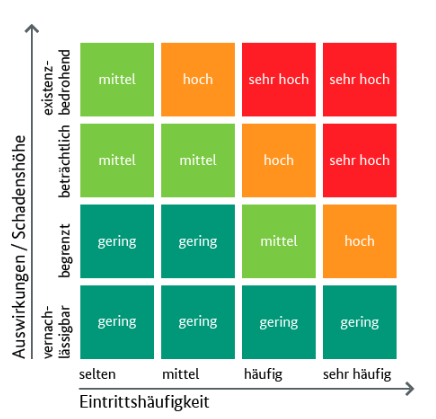
\includegraphics[width=0.6\linewidth]{risikomatrix.png}
    \caption{Beispielhafte Risikomatrix (LL)}
    \label{fig:riskmatrix}
\end{figure}

Die Risikomatrix eignet sich sowohl für die qualitative als auch die quantitive Risikobewertung. Ein Beispiel für ein Instrument, welches sich eher nur für die quantitative Bewertung eignet, ist die Risikowertberechnung:

\begin{quote}
    Sei $P$ die Eintrittswahrscheinlichkeit des Risikos in Prozent, $S$ die Tragweite des Risikos in €. Für den Risikowert $V$ gilt:
    \[ P * S = V \]  
\end{quote}

Dabei ist wichtig zu nennen, dass es keine Methode gibt, die Eintrittswahrscheinlichkeit akkurat zu bestimmen, daher muss die Eintrittswahrscheinlichkeit geschätzt werden. Die Genauigkeit der Schätzung ist dabei von der Erfahrung der schätzenden Personen abhängig. Ähnlich verhält sich die Tragweite. Diese muss ebenfalls oft geschätzt werden, jedoch kann es sein, dass eine genaue Bestimmung möglich ist, je nach Risiko, welches aktuell betrachtet wird.

\subsubsection{Strategien und Maßnahmen zur Risikosteuerung (LL)}
Nach einer Analyse und Bewertung der Risiken kann damit begonnen werden, konkrete Maßnahmen zur Steuerung bzw. Minderung der Risiken zu treffen. Im Groben gibt es vier mögliche Ansätze, wie man mit einem Risiko umgehen kann, die im Folgenden näher behandelt werden. Eine Übersicht der Ansätze ist in Abbildung \ref{fig:riskstrats}\cite[(Section 2)S.~25]{cicek2022risikomanagement} zu finden.

\begin{figure}
    \centering
    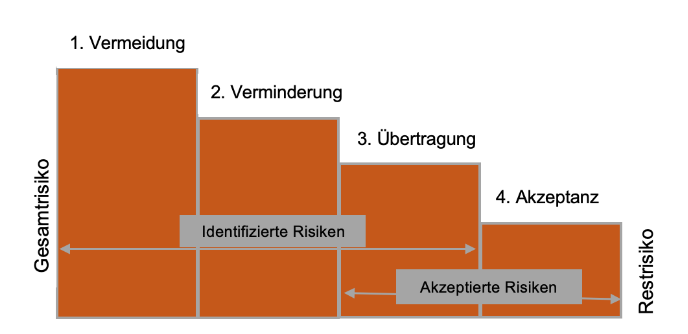
\includegraphics[width=\linewidth]{risiken.png}
    \caption{Mögliche Strategien zur Risikosteuerung nach \cite{cicek2022risikomanagement} (LL)}
    \label{fig:riskstrats}
\end{figure}

\paragraph{Risiko vermeiden (LL)}
Die Vermeidung eines Risikos hat die Absicht, ein Risiko komplett zu umgehen, indem das Eintreten so gut wie möglich verhindert wird. Diese Strategie bietet sich bei besonders schwerwiegenden und als kritisch indentifizierten Risiken an. Eine Vermeidung von allen möglichen Risiken ist nicht möglich, da dies mit sehr hohem Aufwand verbunden ist, der Ressourcen des Projektes bindet welche dann an anderen Stellen fehlen.
Risiken können auf andere verlagert werden. Dabei wird die Eintrittswahrscheinlichkeit des Risikos nicht verändert. Allein die Tragweite im Bezug auf Kosten kann auf Andere (wie zum Beispiel Lieferanten) deligiert werden und mindert das Risiko.


\paragraph{Risiko vermindern (LL)}
Bei der Risikoverminderung ist die Idee, dass man die möglichen Auswirkungen eines Risikos durch früh getroffene Maßnahmen abmildert. Das kann auf verschiedenen Wegen erfolgen, bei Risiken finanzieller Natur können beispielsweise Rücklagen im Budget gebildet werden, welche dann im Eintrittsfall angezapft werden können und damit die Auswirkungen abmildern. Die Risikoverminderung kommt dann zum Einsatz, wenn ein Risiko nicht vermieden werden kann, aber in seinen Auswirkungen trotzdem problematisch ist \cite{dechange_projektmanagement_2024}.

\paragraph{Risiko übertragen (LL)}
Es ist ebenfalls möglich Risiken an dritte Parteien abzutreten. So können bestimmte Tätigkeiten des Projektes an einen externen Dienstleister vergeben werden, welcher die Risikolast vermindert, indem sie auf mehr Parteien verteilt wird. 

\paragraph{Risiko akzeptieren (LL)}
Als letzte Methode bleibt noch, das Risiko zu akzeptieren und nicht weiter zu intervenieren. Das muss insbesondere bei Risiken erfolgen, welche außerhalb des Einflusses des Projekts liegen. Das bedeutet jedoch nicht, diese Risiken einfach zu ignorieren. Sie müssen kontinuierlich überwacht werden, um nicht unvorbereitet im Eintrittsfall zu sein \cite{cicek2022risikomanagement}.

\subsubsection{Risikobudget ermitteln (LL)}
Die Maßnahmen verändern nun den Risikowert der Risiken. Um einschätzen zu können, ob die Maßnahmen sinvoll sind wird der Risikowert vor den Maßnahmen mit dem Risikowert nach den Maßnahmen und den Kosten für die Maßnahmen verglichen. Aus der Summe dieser lässt sich nun das Risikobudget für das Projekt berechnen.

\subsubsection{Risikomanagement im weiteren Projektverlauf (LL)}
Das Risikomanagement ist nicht streng auf die Phase der Projekplanung beschränkt. Zwar ist es enorm hilfreich, Risiken im Voraus zu identifizieren und zu berücksichtigen, jedoch sind im Voraus getroffene Entscheidungen nicht permanent. Risiken sind dynamisch und können sich in ihren Eigenschaften im Verlauf des Projektes verändern. Die Ermittlung und Bewertung der Risiken sollte periodisch im Verlauf des Projektes wiederholt werden, damit man auf Änderungen reagieren kann und nicht unvorbereitet in eine problematische Situation gerät. Dieses Vorgehen wird von \cite[S.~27]{cicek2022risikomanagement} treffend dargestellt, wie in Abbildung \ref{fig:riskcycle} zu sehen ist.

\begin{figure}
    \centering
    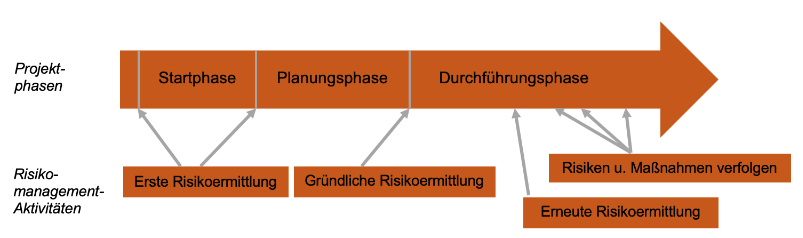
\includegraphics[width=\linewidth]{riskcycle.png}
    \caption{Zyklische Neuevaluiierung der Risiken im Projektablauf (LL)}
    \label{fig:riskcycle}
\end{figure}

\subsubsection{Im Projekt durchgeführtes Risikomanagement (LL)}
Im Vorfeld des Projektes wurde eine Risikoanalyse in einer Sitzung mit allen Mitgliedern durchgeführt. Zunächst wurde mithilfe der Brainstorming-Methode eine Liste an möglichen Risiken angefertigt. Zusammengefasst wurden die folgenden Risiken bestimmt:

\begin{itemize}
    \item Krankheit der Projektmitglieder
    \item Unbekannte Anforderungen an das Softwareprodukt
    \item Vorgaben von höheren Stellen im Unternehmen
    \item Ablehnung des Produktes von Stakeholdern
    \item Lizenzierungsprobleme
\end{itemize}

Ein direktes Risiko, welches berücksichtigt werden muss, ist Ausfall von Projektpersonal durch Krankheit. Dadurch könnte der Projektzeitplan von der Planung abweichen und dadurch Verzögerungen im Ablauf erzeugen oder den Projekterfolg gefährden, wenn der Ausfall längerfristig ist. Ebenfalls problematisch sind Anforderungen an das Produkt, welche vorher nicht korrekt erhoben oder kommuniziert wurden. Diese könnten den Projektablauf zeitlich nach hinten verschieben, da dann bereits untersuchte Kandidaten neu beurteilt werden müssten.

\subsection{Zeit (NW)}
Das Projekt findet in einem fest abgesteckten Zeitraum statt und ist mit einem festen Start- und Enddatum versehen.
Um die vom Kunden gewünschten Lieferobjekte fristgerecht fertigzustellen, wurde sich für eine Planung mithilfe von Meilensteinen mit
Fälligkeitsterminen entschieden. Die Meilensteine wurden daraufhin in einem Planungsmeeting mit allen Mitgliedern des Projektes gefasst und festgehalten.
Eine Aufstellung der Meilensteine ist in Tabelle \ref{tab:milestones} zu finden.\\

Das Projekt ist auf den Zeitraum des Wintersemesters 24/25 an der Hochschule Fulda beschränkt.
Beginn ist der erste Arbeitstag im Semester der Projektmitarbeiter, Ende ist der letzte Arbeitstag des Semesters der Projektmitarbeiter. 
Damit beginnt das Projekt am 15.10.2024 und endet am 04.03.2025. Es umfasst einen Zeitraum von 15 Wochen. 
Die Angaben in diesem Bericht beziehen sich also auf den gesamten Projektverlauf.

\subsection{Stakeholdermanagement (NW)}

Während des Projekts ist ein gutes und kontinuierliches Stakeholdermanagement unerlässlich. 
Bei diesem geht es darum, Personen, Gruppen oder Organisationen zu identifizieren, die durch das Projekt in irgendeiner Weise betroffen sind oder das
Projekt in irgendeiner Weise betreffen und diese in das Projekt mit einzubinden. Wichtig dabei ist es zu analysieren, welche Position 
diese Stakeholder zu dem Projekt haben. Diese können in einer Stakeholdermatrix festgehalten werden. 
Je früher mit dem Stakeholdermanagement begonnen werden kann, desto besser.
Dabei kann folgender Prozess durchlaufen werden \cite[S.~487]{project_management_institute_guide_2017}:

\subsubsection{Stakeholder identifizieren (NW)}
Stakeholder zu identifizieren ist kein einmaliger Prozess. Im Projektverlauf können sich Stakeholder ändern. 
Je nach Phase können neue hinzukommen oder wegfallen. Auch die Einstellung zum Projekt kann sich im Projektverlauf ändern. 
Um auf die Auswirkungen der Stakeholder zu jederzeit reagieren zu können, darf die Identifikation und Analyse der Stakeholder 
zu keiner Zeit vernachlässigt werden.

\subsubsection{Stakeholder Interaktion planen (NW)}
In diesem Schritt wird geplant wie der Kontakt zu Stakeholdern hergestellt werden kann und diese in das Projekt mit eingebunden werden können.\\
Die Planung kann sich dabei an Kategorien wie Einfluss, Postition zum Projekt, Erwartungen oder Interessen orientieren.

\subsubsection{Stakeholder Interaktion Durchführen (NW)}
Im nächsten Schritt wird nun die Kommunikation und Zusammenarbeit mit den Stakeholdern begonnen. 
Dabei sollte über die Erwartungen und Probleme gesprochen werden.

\subsubsection{Stakeholder Interaktion Überwachen (NW)}
Nach den Gesprächen mit den Stakeholdern müssen diese ausgewertet werden, um die Einschätzung der Stakeholder im Bezug auf Einfluss,
Position zum Projekt oder Erwartungen und Interessen zu verbessern.\\
Der Prozess des Stakeholdermanagements ist iterativ angelegt. Die Dokumentation der Stakeholder sollte regelmäßig während
des Projekts stattfinden. Forschungen zum Scheitern von Projekten zeigen die Relevanz des strukturierten Vorgehens 
beim Stakeholdermanagements \cite[S.~488]{project_management_institute_guide_2017}.
Ein besonderes Augenmerk muss auf das Stakeholdermanagement in folgenden Situationen gelegt werden:

\begin{itemize}
	\item Das Projekt erreicht eine neue Phase
	\item Aktuelle Stakeholder sind nicht länger mit dem Projekt verbunden oder neue kommen hinzu
	\item Es gibt signifikante Änderungen in der Organisation des Projekts oder bei Stakeholdern
\end{itemize}
	




\begin{table}[h]
  \centering
\begin{tabular}{|c|c|c|c|c|}
  \hline
  Nummer & Code & Meilsteinname & Basis & Plan \\
  \hline
  1 & MS10 & Projektstart & 14.10.2024 & 14.10.2024 \\
  \hline
  2 & MS20 & Analyse des Ist-Zustandes abgeschlossen & 25.10.2024 & 25.10.2024 \\
  \hline
  3 & MS30 & Anforderungskatalog an Lösung festgelegt & 30.10.2024 & 30.10.2024 \\
  \hline
  4 & MS40 & Auswahl an Produkten zur Ablösung & 06.11.2024 & 06.11.2024 \\
  \hline
  5 & MS50 & Produkte wurden bewertet anhand des Katalogs & 22.11.2024 & 22.11.2024 \\
  \hline
  6 & MS60 & Produktentscheidung steht & 26.11.2024 & 26.11.2024 \\
  \hline
  7 & MS70 & Testumgebung beantragt & 28.11.2024 & 28.11.2024 \\
  \hline
  8 & MS80 & Proof-of-Concept aufgesetzt & 13.12.2024 & 13.12.2024 \\
  \hline
  9 & MS90 & Dokumentation angefertigt & 14.01.2025 & 14.01.2025 \\
  \hline
  10 & MS100 & Ergebnisse dem Kunden vorgestellt & 24.01.2025 & 24.01.2025 \\
  \hline
  11 & MS110 & Projekt-Retrospektive & 28.01.2025 & 28.01.2025 \\
  \hline
  12 & MS120 & Ende des Projektes & 31.01.2025 & 31.01.2025 \\
  \hline
\end{tabular}

  \caption{Meileinsteine des Projekts (LL)}
\label{tab:milestones}

\end{table}

\end{document}
